\chapter{Tips and Tricks}

\begin{itemize}
\item Either install Latex on your own machine, maybe in a docker-image, or use overleaf. \\
    On your own machine, the compilation will commence more quickly. There is also no compilation timeout, which you may run into with overleaf.
\item actively use $\backslash$include (for chapters) and $\backslash$input to break you 
 big document into smaller parts. If you then have a file called IncludeOnly.tex in your root dir, only the chapters in that file will be included. In this way it is easy to make something for your reviewers, but also speeds up the compilation process drastically, which is nice while you are editing and you work (re)view-driven.
\item If you add pictures or tables, always choose vector format. Never jpeg unless it is a photo, png only for screenshots, which you should try to avoid. In the drawing tool (Visual Paradigm, Umlet, drawio)  you can most likely export in pdf format which you can include with $\backslash$includegraphics. If you have svg, which the other popular vector format, you can use a conversion tool to turn it into a pdf. Inkscape, which is available on all relevant platforms, does the trick for me.
For tables, a spreadsheet(excel libreoffice calc) is a reasonable choice. Export the selection as pdf with no borders. May use a tool to clip/crop off the white borders. pdfcrop works for me there.
\end{itemize}

\begin{figure}[htbp]
\caption{Example svg image}
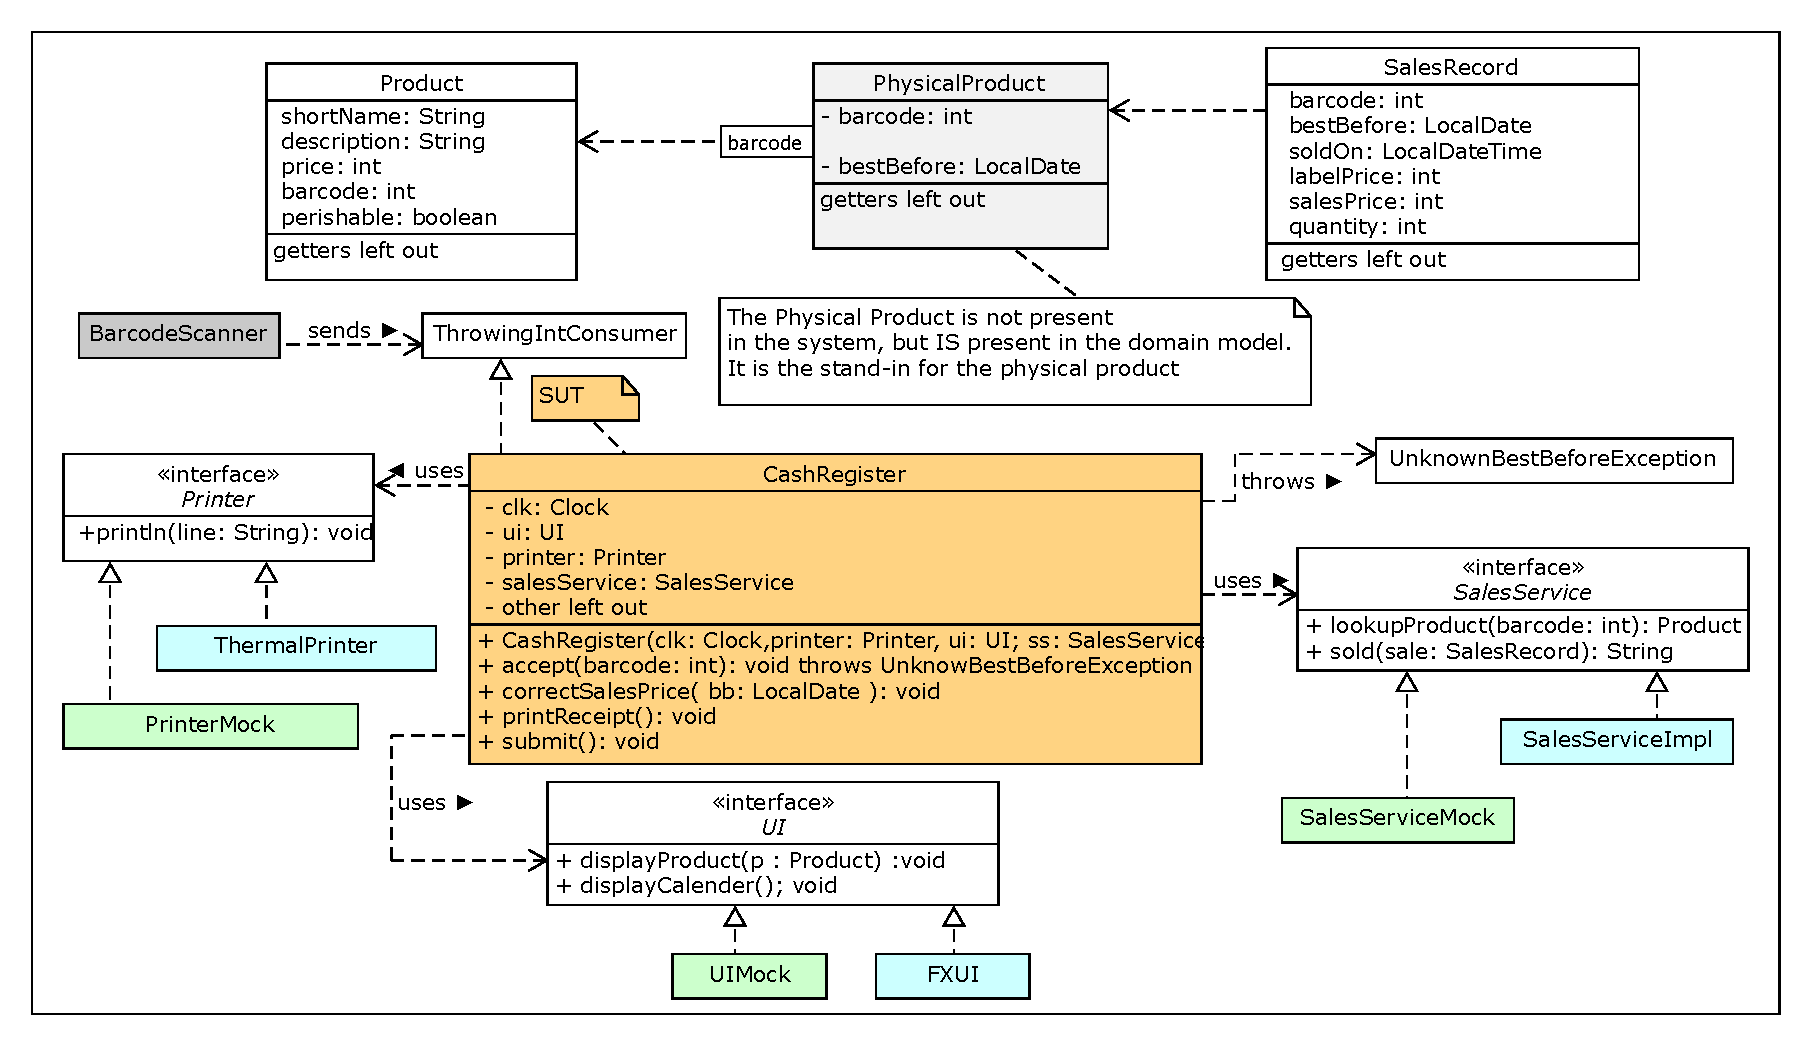
\includegraphics[width=\linewidth]{images/perishablesales.pdf}
\end{figure}

Try to select text in the image and zoom in and the advantages become apparent.